\documentclass[14pt,a4paper]{extarticle}

\usepackage{fontspec}
\setmainfont{Times New Roman}
\setsansfont{Helvetica}
\usepackage{polyglossia}
\setdefaultlanguage{russian}
\setotherlanguage{english}
\newfontfamily\russianfonttt{Courier New}

\usepackage[left=30mm,right=15mm,top=20mm,bottom=20mm]{geometry}
\usepackage{setspace}
\onehalfspacing
\usepackage{indentfirst}
\setlength{\parindent}{1.25cm}

\tolerance=9000
\emergencystretch=3em
\hbadness=10000
\setlength{\overfullrule}{0pt}

\usepackage{graphicx}
\usepackage{float}

\usepackage{caption}
\captionsetup[figure]{name=Рисунок,labelsep=endash}

\usepackage{fancyhdr}
\pagestyle{fancy}
\fancyhf{}
\fancyfoot[C]{\thepage}
\renewcommand{\headrulewidth}{0pt}

\usepackage[hidelinks]{hyperref}

\usepackage{listings}
\lstset{
  basicstyle=\small\ttfamily,
  breaklines=true,
  frame=single,
  xleftmargin=1.25cm,
  numbers=left,
  numberstyle=\tiny,
  showstringspaces=false,
  tabsize=4,
}

\begin{document}

\thispagestyle{empty}
\begin{center}
\textbf{МИНИСТЕРСТВО НАУКИ И ВЫСШЕГО ОБРАЗОВАНИЯ РОССИЙСКОЙ ФЕДЕРАЦИИ}\\[0.3cm]
\textbf{УНИВЕРСИТЕТ ИТМО}\\[0.5cm]
Факультет ПИиКТ\\[1.5cm]

\textbf{\Large Лабораторная работа №1}\\[0.5cm]
\textbf{\large Разработка десктопного приложения на Avalonia UI}\\[0.5cm]
по дисциплине <<Создание программного обеспечения>>\\[2cm]
\end{center}

\begin{flushleft}
\hspace{1.25cm}\begin{minipage}[t]{\dimexpr\textwidth-1.25cm\relax}
\textbf{Выполнил:} студент Луценко Владимир\\
\textbf{Группа:} К3420\\
\textbf{Преподаватель:} Осипов Н. А.\\
\end{minipage}
\end{flushleft}

\vfill
\begin{center}
Санкт-Петербург, 2026
\end{center}
\newpage

\tableofcontents
\newpage

\section{Введение}

Цель работы -- освоение разработки десктопных приложений на платформе .NET. В рамках лабораторных работ 1--8 реализован калькулятор с расширенными математическими функциями, а также ряд учебных приложений, демонстрирующих работу с формами, контролами, диалогами, графикой и асинхронностью. В качестве UI-фреймворка использован Avalonia -- кросс-платформенный аналог WPF, поддерживающий XAML-разметку и работающий на Windows, macOS и Linux.

\section{ЛР 1--2. Формы и контролы}

Создан проект калькулятора на базе Avalonia UI. Интерфейс описан в XAML-файле \texttt{MainWindow.axaml} с использованием \texttt{Grid} для компоновки кнопок. Вычислительная логика вынесена в отдельный класс \texttt{CalcEngine}.

\begin{lstlisting}[caption={XAML-разметка калькулятора (фрагмент)},language=xml]
<Window Title="Калькулятор"
        Width="320" Height="480"
        CanResize="False">
  <Grid RowDefinitions="Auto,*" Margin="8">
    <TextBox Name="Display" Grid.Row="0"
             FontSize="28" IsReadOnly="True"
             TextAlignment="Right" Text="0"/>
    <Grid Grid.Row="1"
          RowDefinitions="*,*,*,*,*,*"
          ColumnDefinitions="*,*,*,*">
      <Button Content="7" Click="OnNumber"/>
      <Button Content="+" Click="OnOperator"
              Classes="op"/>
      <Button Content="=" Click="OnEqual"
              Classes="eq"/>
    </Grid>
  </Grid>
</Window>
\end{lstlisting}

\begin{figure}[H]
\centering
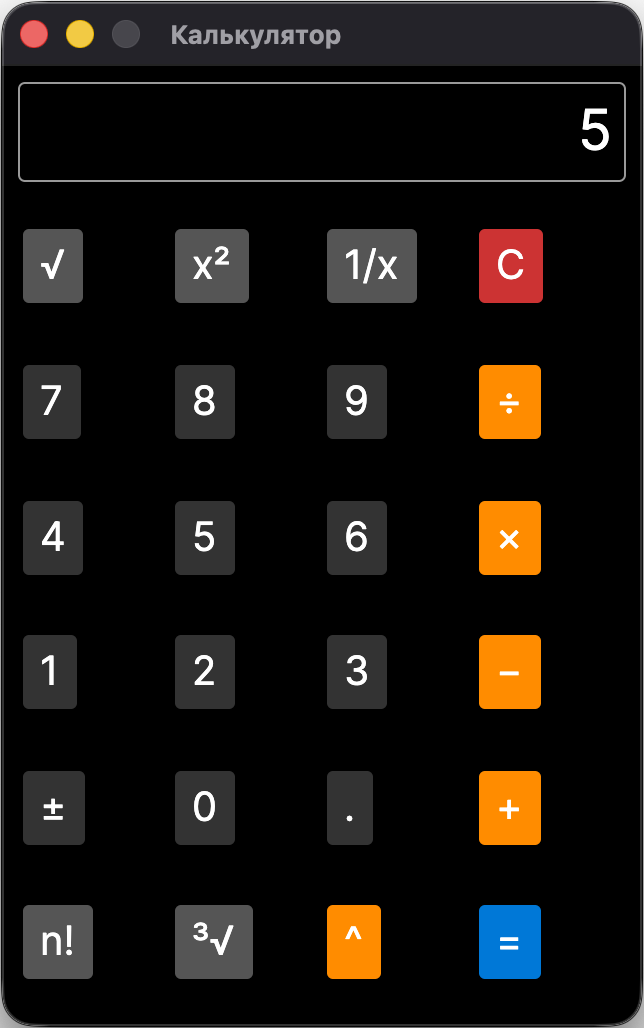
\includegraphics[width=0.4\textwidth]{../../скрины/SCR-20260328-pyog.png}
\caption{Калькулятор на Avalonia UI (macOS)}
\end{figure}

Форма калькулятора имеет фиксированный размер (\texttt{CanResize="False"}) -- аналог свойства \texttt{FormBorderStyle = FixedSingle} в WinForms. Стили кнопок заданы через \texttt{Window.Styles} с использованием CSS-подобных селекторов Avalonia.

\begin{lstlisting}[caption={Обработчики кнопок в code-behind},language={[Sharp]C}]
// Нажатие цифры
private void OnNumber(object? sender, RoutedEventArgs e)
{
    var btn = (Button)sender!;
    var result = CalcEngine.CalcNumber(
        btn.Content!.ToString()!);
    Display.Text = result;
}

// Выбор оператора (+, -, *, /, ^)
private void OnOperator(object? sender, RoutedEventArgs e)
{
    var btn = (Button)sender!;
    var op = btn.Content!.ToString() switch
    {
        "+" => CalcEngine.Operator.eAdd,
        _ => CalcEngine.Operator.eUnknown
    };
    CalcEngine.CalcOperation(op);
}
\end{lstlisting}

\section{ЛР 3--4. Пользовательские контролы и диалоги}

Реализованы пользовательские контролы: \texttt{NumericTextBox} (ввод только цифр), \texttt{ColorPicker} (выбор цвета), \texttt{HighlightButton} (кнопка с подсветкой при наведении). Диалоговые окна реализованы как отдельные \texttt{Window}: модальное окно вызывается через \texttt{ShowDialog(owner)}, немодальное -- через \texttt{Show()}.

\begin{lstlisting}[caption={Модальное и немодальное окно},language={[Sharp]C}]
// Модальное окно -- блокирует родительское
var dialog = new SettingsDialog();
await dialog.ShowDialog(this);

// Немодальное окно -- не блокирует
var window = new FindDialog();
window.Show();
\end{lstlisting}

\section{ЛР 5. Вычислительный движок CalcEngine}

Класс \texttt{CalcEngine} содержит всю математическую логику калькулятора. Реализованы базовые операции (сложение, вычитание, умножение, деление, возведение в степень) и расширенные функции.

\begin{lstlisting}[caption={Расширенные математические функции},language={[Sharp]C}]
// Квадратный корень
public static string CalcSqrt()
{
    if (stringAnswer != "")
    {
        double num = Convert.ToDouble(stringAnswer);
        if (num >= 0)
            numericAnswer = Math.Sqrt(num);
        else
            stringAnswer = "Error";
    }
    return stringAnswer;
}

// Факториал
public static string CalcFactorial()
{
    int n = Convert.ToInt32(
        Convert.ToDouble(stringAnswer));
    long result = 1;
    for (int i = 2; i <= n; i++)
        result *= i;
    numericAnswer = result;
    stringAnswer = Convert.ToString(numericAnswer);
    return stringAnswer;
}
\end{lstlisting}

Также реализованы: квадрат числа (\texttt{CalcSquare}), обратное число (\texttt{CalcReciprocal}), кубический корень (\texttt{CalcCubeRoot}) и решение квадратного уравнения (\texttt{SolveQuadratic}).

\section{ЛР 6. Графика}

Реализовано приложение с тремя панелями: построение графика функции, диаграмма и анимация. Для отрисовки используется \texttt{GDI+} через обработчик \texttt{Paint} с объектом \texttt{Graphics}. Панель графика строит синусоиду по точкам методом \texttt{DrawLines}, панель диаграммы отображает столбчатую диаграмму через \texttt{FillRectangle}, панель анимации перемещает фигуру с помощью \texttt{Timer}.

\section{ЛР 7. Асинхронность}

Реализована асинхронная загрузка данных с использованием \texttt{async/await} и \texttt{Task.Run}. Длительная операция выполняется в фоновом потоке, UI остаётся отзывчивым. Прогресс отображается через \texttt{ProgressBar}, обновление UI происходит через диспетчер.

\begin{lstlisting}[caption={Асинхронная загрузка},language={[Sharp]C}]
private async void OnLoadClick(object sender,
    EventArgs e)
{
    progressBar.Value = 0;
    btnLoad.Enabled = false;

    await Task.Run(() =>
    {
        for (int i = 0; i <= 100; i++)
        {
            Thread.Sleep(50);
            Invoke(() => progressBar.Value = i);
        }
    });

    btnLoad.Enabled = true;
    MessageBox.Show("Загрузка завершена!");
}
\end{lstlisting}

\section{ЛР 8. Юзабилити}

Реализованы улучшения интерфейса: горячие клавиши (\texttt{KeyDown}), всплывающие подсказки (\texttt{ToolTip}), валидация ввода, обработка ошибок с информативными сообщениями. Калькулятор корректно обрабатывает деление на ноль и извлечение корня из отрицательного числа.

\section{Заключение}

В ходе лабораторных работ 1--8 разработан калькулятор с расширенным набором математических функций. Использован фреймворк Avalonia UI, позволяющий запускать приложение на Windows, macOS и Linux из единого кода. Интерфейс описан в XAML, логика вынесена в отдельный класс \texttt{CalcEngine}. Реализованы пользовательские контролы, диалоговые окна, графика, асинхронные операции и улучшения юзабилити.

\end{document}
